% This is a LaTeX input file.
%
% A '%' character causes TeX to ignore all remaining text on the line,
% and is used for comments like this one.

\documentclass[a4paper,notitlepage]{article}      % Specifies the document class
                            % The preamble begins here.
\title{Interpretation of Somers'~$D$ under four simple models}  % Declares the document's title.
\author{Roger B. Newson}      % Declares the author's name.
\date{06 July, 2022}      % Deleting this command produces today's date.

\usepackage{fancyhdr}
\usepackage{lastpage}
\usepackage{graphics}
\usepackage{hyperref}

%\newcommand{\ip}[2]{(#1, #2)}
                             % Defines \ip{arg1}{arg2} to mean
                             % (arg1, arg2).

%\newcommand{\ip}[2]{\langle #1 | #2\rangle}
                             % This is an alternative definition of
                             % \ip that is commented out.

%
% Set margins
% (which are explained in Figure C3 of LaTeX User's Guide
% and which CAN BE RESET BY EDITORS AT ANY TIME AS FAR AS I CARE!!!!!!!!
% - RBN.)
%
\setlength{\topmargin}{-0.5in}
%\setlength{\headsep}{0.25in}
\setlength{\oddsidemargin}{0in}
\setlength{\evensidemargin}{0in}
\setlength{\textwidth}{6.5in}
\setlength{\textheight}{10in}

%
% Set page style (headers and footers)
%
\pagestyle{fancy}
\fancyhf{}
\fancyhead[LO,LE]{\textit{Interpretation of Somers'~$D$ under four simple models. Page \thepage\ of \pageref{LastPage}.}}
\fancyfoot[LO,LE]{}

\begin{document}             % End of preamble and beginning of text.

\maketitle                   % Produces the title.

\section{Introduction}

Somers'~$D$ is an ordinal measure of association introduced by Somers (1962)\cite{somers1962}.
It can be defined in terms of Kendall's $\tau_a$ (Kendall and Gibbons, 1990)\cite{kendall1990}.
Given a sequence of bivariate random variables $(X,Y)=\{(X_i,Y_i)\}$,
sampled using a sampling scheme for sampling pairs of bivariate pairs
from a population of pairs of bivariate pairs,
Kendall's $\tau_a$ is defined as
\def\sign{{\rm sign}}
\begin{equation}
\tau(X,Y)=E\left[\sign(X_i-X_j)\sign(Y_i-Y_j)\right]
\label{eq:eqseq15}
\end{equation}
(where $E[\cdot]$ denotes expectation), or, equivalently,
as the difference between the probability that the two $X,Y$--pairs are concordant
and the probability that the two $X,Y$--pairs are discordant.
A pair of $X,Y$--pairs is said to be concordant if the larger $X$--value is paired with the larger $Y$--value,
and is said to be discordant if the larger $X$--value is paired with the smaller $Y$--value.
Somers'~$D$ of $Y$ with respect to $X$ is defined as
\begin{equation}
D(Y|X)=\tau(X,Y)/\tau(X,X)
\label{eq:eqseq16}
\end{equation}
or, equivalently, as the difference between the two \textit{conditional} probabilities of concordance and discordance,
assuming that the 2 $X$--values are unequal.
Note that Kendall's $\tau_a$ is symmetric in $X$ and $Y$,
whereas Somers'~$D$ is asymmetric in $X$ and $Y$.

Somers'~$D$ plays a central role in rank statistics,
and is the parameter behind most of these ``nonparametric'' methods,
and can be estimated with confidence limits like other parameters.
It can also be generalized to sampling--probability weighted and/or clustered and/or possibly censored data.
(See Newson (2002)\cite{newson2002} and Newson (2006)\cite{newson2006} for details.)
However, many non--statisticians appear to have a problem interpreting Somers'~$D$,
even though a difference between proportions is arguably a simpler concept than an odds ratio,
which many of them claim to understand better.
Parameters are often easier to understand if they play a specific role in a specific model.
Fortunately, in a number of simple standard models,
Somers'~$D$ can be derived from another parameter by a transformation.
A confidence interval for Somers'~$D$ can therefore be transformed, using inverse end--point transformation,
to give a robust, outlier--resistant confidence interval for the other parameter,
assuming that the model is true.

We will discuss 4 simple models for bivariate $X,Y$--pairs:

\begin{itemize}

\item \textbf{Binary $X$, binary $Y$.} Somers'~$D$ is then the difference between proportions.

\item \textbf{Binary $X$, continuous $Y$, constant hazard ratio.} Somers'~$D$ is then a transformation of the hazard ratio.

\item \textbf{Binary $X$, Normal $Y$, equal variances.}
Somers'~$D$ is then a transformation of the mean difference divided by the common standard deviation (SD).
(Or, equivalently, a transformation of an interpercentile odds ratio of $X$ with respect to $Y$.)

\item \textbf{Bivariate Normal $X$ and $Y$.} Somers'~$D$ is then a transformation of the Pearson correlation coefficient.

\end{itemize}

Each of these cases has its own Section, and a Figure (or Figures) illustrating the transformation.
In each case, the alternative parameter (or its log) is nearly a linear function of Somers'~$D$,
for values of Somers'~$D$ between -0.5 and 0.5.

\section{Binary $X$, binary $Y$}

We assume that there are two subpopulations, Subpopulation~$A$ and Subpopulation~$B$, and that $X$ is a binary indicator variable,
equal to 1 for observations in Subpopulation~$A$ and 0 for observations in Subpopulation~$B$,
and that $Y$ is also a binary variable, equal to 1 for ``successful'' observations and 0 for ``failed'' observations.
Define
\def\Pr{{\rm Pr}}
\begin{equation}
p_A \, = \, \Pr(Y=1|X=1), \quad p_B \, = \, \Pr(Y=1|X=0)
\label{equation:eqseq17}
\end{equation}
to be the probabilities of ``success'' in Subpopulations~$A$ and $B$, respectively. Then Somers'~$D$ is simply
\begin{equation}
D(Y|X) \, = \, p_A \, - \, p_B ,
\label{equation:eqseq18}
\end{equation}
or the difference between the two probabilities of ``success''.
Figure~\ref{figure:figseq1} gives Somers'~$D$ as the trivial identity function of the difference between proportions.
Note that Somers'~$D$ is expressed on a linear scale of multiples of 1/12,
which (as we will see) is arguably a natural scale of reference points for Somers'~$D$.

\section{Binary $X$, continuous $Y$, constant hazard ratio}

We assume, again, that $X$ indicates membership of Subpopulation~$A$ instead of Subpopulation~$B$,
and assume, this time, that $Y$ has a continuous distribution in each of the two subpopulations,
with cumulative distribution functions $F_A(\cdot)$ and $F_B(\cdot)$,
and probability density functions $f_A(\cdot)$ and $f_B(\cdot)$.
We imagine $Y$ to be a survival time variable,
although we will not consider the possibility of censorship.
In the two subpopulations, the survival functions and the hazard functions are given, respectively, by
\begin{equation}
S_k(y) \, = \, 1-F_k(y), \quad h_k(y) = f_k(y)/S_k(y),
\label{equation:eqseq19}
\end{equation}
where $y$ is in the range of $Y$ and $k\in \{A,B\}$.
Suppose that the hazard ratio $h_A(y)/h_B(y)$ is constant in $y$,
and denote its value as $R$.
(This is trivially the case if both subpopulations have an exponential distribution,
with $h_k(y)=1/\mu_k$, where $\mu_k$ is the subpopulation mean.
However, it can also be the case if we assume some other distributional families,
such as the Gompertz or Weibull families,
or even if we do not assume any specific distributional family,
but still assume the proportional hazards model of Cox (1972)\cite{cox1972}.)
Somers'~$D$ is then derived as
\begin{equation}
D(Y|X) \, = \, {
{ \int_y h_B(y) S_A(y) S_B(y) dy \, - \, \int_y R \, h_B(y) S_A(y) S_B(y) dy }
\over
{ \int_y h_B(y) S_A(y) S_B(y) dy \, + \, \int_y R \, h_B(y) S_A(y) S_B(y) dy }
}
\, = \, (1-R)/(1+R) .
\label{eq:eqseq20}
\end{equation}
Note that Somers'~$D$ is then the parameter that is zero under the null hypothesis tested using the method of
Gehan (1965)\cite{gehan1965}.
For finite $R$, this formula can be inverted to give the hazard ratio $R$ as a function of Somers'~$D$ by
\begin{equation}
R \, = \, \left[ 1 - D(Y|X) \right] / \left[ 1 + D(Y|X) \right] = \left[ 1 - c(Y|X) \right]/c(Y|X) ,
\label{eq:eqseq21}
\end{equation}
where $c(Y|X)=[D(Y|X)+1]/2$ is Harrell's $c$-index,
which reparameterizes Somers'~$D$ to a probability scale from 0 to 1 (Harrell \textit{et al.}, 1982)\cite{harrell1982}.
Note that, for continuous $Y$ and binary $X$, Harrell's~$c$ is the probability of concordance,
and that a constant hazard ratio $R$ is the corresponding odds \textit{against} concordance.

Figure~\ref{figure:figseq2} gives Somers'~$D$ as a function of $R$.
Note that $R$ is expressed on a log scale, similarly to the standard practice with logistic regression.
Somers'~$D$ of lifetime with respect to membership of Population~$A$
is seen to be a decreasing logistic sigmoid function of the Population~$A$/Population~B log hazard ratio,
equal to 0 when the log ratio is 0 and the ratio is therefore 1.
A hazard ratio of 2 (as typically found when comparing the lifetimes of cigarette smokers as Population~A to lifetimes of nonsmokers as Population~B)
corresponds to a Somers'~$D$ of -1/3, or a Harrell's~$c$ of 1/3.
Similarly, a hazard ratio of 1/2 (as typically found when comparing lifetimes of nonsmokers as Population~$A$ to lifetimes of cigarette smokers as Population~$B$)
corresponds to a Somers'~$D$ of 1/3, or a Harrell's~$c$ of 2/3.
Therefore, although a smoker may possibly survive a non--smoker of the same age,
the odds are 2 to 1 against this happening. A hazard ratio of 3 corresponds to a Somers'~$D$ of -0.5,
and a hazard ratio of 1/3 corresponds to a Somers'~$D$ of 0.5.
For even more spectacular hazard ratios in either direction,
the linearity breaks down, even though the hazard ratio is logged.

\section{Binary $X$, Normal $Y$, equal variances}

We assume, again, that $X$ indicates membership of Subpopulation~$A$ instead of Subpopulation~$B$,
and assume, this time, that $Y$ has a Normal distribution in each of the two subpopulations,
with respective means $\mu_A$ and $\mu_B$
and standard deviations (SDs) $\sigma_A$ and $\sigma_B$.
Then, the probability of concordance (Harrell's~$c$)
is the probability that a random member of Population~$A$ has a higher $Y$--value than a random member of Population~$B$,
or (equivalently) the probability that the difference between these two $Y$--values is positive.
This difference has a Normal distribution, with mean $\mu_A-\mu_B$ and variance $\sigma_A^2+\sigma_B^2$.
Somers'~$D$ is therefore given by the formula
\begin{equation}
D(Y|X) \, = \, 2\Phi\left({{\mu_A-\mu_B}\over{\sqrt{\sigma_A^2+\sigma_B^2}}}\right) \, - \, 1,
\label{equation:eqseq22}
\end{equation}
where $\Phi(\cdot)$ is the cumulative standard Normal distribution function.
If the two SDs are both equal (to $\sigma=\sigma_A=\sigma_B$), then this formula simplifies to
\begin{equation}
D(Y|X) \, = \, 2\Phi\left({{\mu_A-\mu_B}\over{\sigma\sqrt{2}}}\right) \, - \, 1 \, = \, 2\Phi\left(\delta\over {\sqrt{2}}\right) \, - \, 1,
\label{eq:eqseq23}
\end{equation}
where $\delta=(\mu_A-\mu_B)/\sigma$ is the difference between the two means,
expressed in units of the common SD.
The parameter $\delta$ can therefore be defined as a function of Somers'~$D$ by the inverse formula
\begin{equation}
\delta \, = \, \sqrt{2} \Phi^{-1}\left( {{D(Y|X)+1}\over 2 } \right),
\label{equation:eqseq24}
\end{equation}
where $\Phi^{-1}(\cdot)$ is the inverse standard Normal cumulative distribution function.

Figure~\ref{figure:figseq3} gives Somers'~$D$ as a function of the mean difference, expressed in SD units.
Again, we see a sigmoid curve, but this time Somers'~$D$ is increasing with the alternative parameter.
Note that a mean difference of 1 SD corresponds to a Somers'~$D$ just above 1/2 (approximately 52049988),
corresponding to a concordance probability (or Harrell's~$c$) just above 3/4,
whereas a mean difference of -1 SDs corresponds to a Somers'~$D$ of just below -1/2 (approximately -.52049988),
or a Harrell's~$c$ just below 1/4.
For mean differences between -1 SD and 1 SD,
the corresponding Somers'~$D$ can be interpolated (approximately) in a linear fashion,
with Somers'~$D$ approximately equal to half the mean difference in SDs.
A mean difference of 2 SDs corresponds to a Somers'~$D$ of approximately .84270079 (slightly more than 5/6),
or a Harrell's~$c$ of approximately .9213504 (slightly over 11/12).
A mean difference of 3 SDs corresponds to a Somers'~$D$ of approximately .96610515 (slightly more than 19/20),
or a Harrell's~$c$ of .98305257 (over 49/50).
For mean differences over 3 SDs, the probability of discordance falls to fractions of a percent,
and Somers'~$D$ becomes progressively less useful,
as there is very little overlap between subpopulations for Somers'~$D$ to measure.
Within the range of approximate linearity ($\pm 1$ SDs),
a Somers'~$D$ of 0, $\pm 1/4$, $\pm 1/3$ or $\pm 1/2$ corresponds to a difference of
0, $\pm .45062411$, $\pm .60914039$ or $\pm .95387255$ SDs, respectively.

Note that the above argument applies equally if $Y$ is calculated
using a Normalizing and variance--stabilizing monotonic transformation
on an untransformed variable whose distribution is not Normal.
As Somers'~$D$ is a rank parameter,
it is preserved by monotonically--increasing transformations.
Therefore, \textit{if} a Normalizing and variance--stabilizing increasing transformation exists,
\textit{then} we can estimate $\delta$
from the Somers'~$D$ of the untransformed variable with respect to the binary $X$
by end--point transformation of Somers~$D$ and its confidence limits,
using (\ref{equation:eqseq24}).
This can be done without even knowing the Normalizing and variance--stabilizing transformation.
Therefore, a lot of work can be saved this way,
if it was the mean difference in SDs that we wanted to know.

\subsection{Likelihood and odds ratios for diagnostic and case--control data}

The equal--variance Normal model is also often used as a ``toy model''
for the problem of defining diagnostic tests, based on a continuous marker variable $Y$,
for membership of Subpopulation~$A$ instead of Subpopulation~$B$.
In this case, Subpopulation~$A$ might be diseased individuals,
Subpopulation~$B$ might be non--diseased individuals,
and $Y$ might be a quantitative test result.
If the true distribution of $Y$ in each subpopulation is Normal,
with a common subpopulation variance and different subpopulation means,
then the log of the likelihood ratio between Subpopulations~$A$ and $B$ is a linear function of the $Y$-value,
given by the formula
\def\LR{{\rm LR}}
\begin{equation}
\log \LR \, = \, {{\mu_B^2 - \mu_A^2}\over{2 \sigma^2}} \, + \, \left( {{\mu_A-\mu_B}\over{\sigma^2}} \right) Y .
\label{equation:eqseq25}
\end{equation}
Note that the intercept term is the value of the log likelihood ratio if $Y=0$,
whereas the slope term is equal to $\delta/\sigma$ in our notation.
Therefore, $\delta$, the mean difference expressed in standard deviations,
is the slope of $\log \LR$ with respect to $Y/\sigma$,
the $Y$--value expressed in standard deviations.
In Bayesian inference, this log likelihood ratio is added to the log of the prior (pre--test) odds of membership
of Subpopulation~$A$ instead of Subpopulation~$B$,
to derive the log of the posterior (post--test) odds of membership
of Subpopulation~$A$ instead of Subpopulation~$B$.
The role of Somers'~$D$ in diagnostic tests is discussed in Newson (2002)\cite{newson2002}.
Briefly, if we graph true--positive rate (sensitivity) against false--positive rate (1$-$specificity),
and choose points on the graph corresponding to the various possible test thresholds,
and join these points in ascending order of candidate threshold value,
then the resulting curve is known as the sensitivity--specificity curve,
or (alternatively) as the receiver--operating characteristic (ROC) curve.
Harrell's~$c$ is the area below the ROC curve,
whereas Somers'~$D$ is the difference between the areas below and above the ROC curve.
The likelihood ratio is the slope of the ROC curve
(defined as the derivative of true--positive rate with respect to false--positive rate),
and, in the equal--variance Normal model, is computed by exponentiating (\ref{equation:eqseq25}).
The equal--variance Normal model, predicting the test result from the disease status,
is therefore combined with Bayes' theorem to imply a logistic regression model
for estimating the disease status from the test result.
Figure~\ref{figure:figseq3} therefore implies (unsurprisingly)
that, other things being equal,
the ROC curve becomes higher as the mean difference (in SDs) becomes higher.

The equal--variance Normal ``toy model'' is also useful for interpreting case--control studies.
In these studies, Subpopulation~$A$ is the cases, Subpopulation~$B$ is the controls,
and $Y$ is a continuous disease predictor.
The rare--disease assumption implies that the distribution of $Y$ in the controls
is a good approximation to the distribution of $Y$ in the population,
and that a population relative risk can be estimated using the corresponding odds ratio.
The 100$q$th percentile of $Y$ in the control population is then $\xi_q=\mu_B+\sigma\Phi^{-1}(q)$
for $q$ in the interior of the unit interval.
It follows from (\ref{equation:eqseq25}) that, for $q<0.5$,
the log of the interpercentile odds ratio between $\xi_{1-q}$ and $\xi_q$
is defined as the difference between the log likelihood ratios at $\xi_{1-q}$ and $\xi_q$.
If we express $Y$ in SD units, then, by (\ref{equation:eqseq25}), this difference is given by
\def\OR{{\rm OR}}
\begin{equation}
\log \OR_q \, = \, \delta \left[ \Phi^{-1}(1-q) - \Phi^{-1}(q) \right] \, = \, 2 \delta \Phi^{-1}(1-q).
\label{equation:eqseq28}
\end{equation}
For instance, if $q=1/4=0.25$, then $\OR_q$ is the interquartile odds ratio,
equal to
\begin{equation}
\OR_{0.25} \, = \, \exp \left\{ \, \delta \left[ \Phi^{-1}(0.75) - \Phi^{-1}(0.25) \right] \, \right\}
\, = \, \exp \left[ 2 \delta \Phi^{-1}(0.75) \right].
\label{equation:eqseq29}
\end{equation}

The plot of Somers'~$D$ against the interquartile odds ratio $\OR_{0.25}$ (on a log scale)
is given as Figure~\ref{figure:figseq5}.
A Somers'~$D$ of 1/12, 1/6, 1/4, 1/3, 5/12 or 1/2 is equivalent to an interquartile odds ratio
of 1.2209313, 1.4939801, 1.8365388, 2.2744037, 2.847498 or 3.6210155, respectively.
Again, this argument is still valid if $Y$ is derived from an original non--Normal variable,
using  a Normalizing and variance--stabilizing monotonically--increasing transformation.
And, again, Somers'~$D$ can be estimated from the original untransformed variable,
without knowing the transformation.

In the range of Somers'$D$ values from -0.5 to 0.5,
the relationship between Somers'~$D$ and the log of the interpercentile odds ratio
is approximmately linear
(see Figure~\ref{figure:figseq5} and observe the linearity from interquartile odds ratios $1/4=0.25$ to 4),
corresponding approximately to Somers'~$D$ from -0.5 to 0.5).
From (\ref{equation:eqseq28}) and (\ref{equation:eqseq24}), we have for $q\in(0,1)$,
\begin{equation}
\log \OR_q \, = \, 2\sqrt{2}\Phi^-1(1-q) \Phi^{-1} \left(  {{D(Y|X)+1}\over 2} \right)
\, = \, 2\sqrt{2} \Phi^{-1}(1-q) \Phi^{-1} \left[ c(Y|X) \right],
\label{equation:eqseq30}
\end{equation}
where $c(Y|X)=[D(Y|X)+1]/2$ is Harrell's~$c$ of $Y$ with respect to $X$
(Harrell {\it et al.}, 1982)\cite{harrell1982}.
For $c(Y|X) \in [0.25, 0.75]$ (corresponding to $D(Y|X) \in [-0.5,0.5]$),
\ref{equation:eqseq30}) can be aproximated linearly by the interpolation formula
\begin{equation}
\log \OR_q \, \approx \,
4 \sqrt{2} \Phi^{-1}(1-q) \left\{ \left[ c(Y|X) - 0.25 \right] \Phi^{-1}(0.75) \, + \, \left[ 0.75 - c(Y|X) \right] \Phi^{-1}(0.25)  \right\} .
\label{equation:eqseq31}
\end{equation}
Figure~\ref{figure:figseq6} shows the exact and approximate interquartile range
(implied by exponentiating (\ref{equation:eqseq31}))
as a function of Harrell's~$c$ under the two--sample equal--variance Normal model.
Note that the horizontal axis is labelled at non--negative multiples of $k/24$ for Harrell's~$c$,
corresponding to the possibly--negative multiples of $k/12$ for Somers'~$D$
Note that the dotted line for the approximate formula
is a good approximation to the exact formula for Harrell's~$c$ from 0.25 to 0.75,
but not outside that range.

This formula can be useful in interpreting differences between Harrell's~$c$ indices for different predictors.
If we have 2 predictors $Y$ and $Z$,
then confidence intervals for differences between $D(Y|X)$ and $D(Z|X)$,
or for differences between $c(Y|X)$ and $c(Z|X)$,
may be used to eliminate the possibility that a positive association between $Y$ and $X$ might be secondary
to a positive association of both $X$ and $Y$ with $Z$.
(See Newson (2006)\cite{newson2006} and Newson (2002)\cite{newson2002}.)
Unfortunately, a lot of statistically--minded scientists think that they understand odds ratios (and their ratios),
but do not think that they understand Somers'~$D$ and Harrell's~$c$ (and their differences).
To prevent culture shock in such scientists,
we can re--interpret the difference between Harrell's~$c$ indices in terms of ratios of odds ratios,
at least if the Harrell's~$c$ indices being compared are between 0.25 and 0.75,
and if we also assume that $Y$ and $Z$ can both be transformed to standard Normal variables.
For $q \in (0,1)$,
define $\OR_q(Y|X)$ as the odds ratio for $X$ between percentiles $100(1-q)$ and $100q$ of $Y$,
and define $\OR_q(Z|X)$ as the odds ratio for $X$ between percentiles $100(1-q)$ and $100q$ of $Z$.
From (\ref{equation:eqseq31}), we have the linear approximation
\begin{equation}
\log \left[ \OR_q(Y|X) / \OR_q(Z|X) \right] \, \approx \,
8 \sqrt{2} \Phi^{-1}(1-q) \Phi^{-1}(0.75) \left[ c(Y|X) - c(Z|X) \right] .
\label{equation:eqseq32}
\end{equation}
This parameter is a ratio between odds ratios, and implies, in the case of a ratio between interquartile ratios, that
\begin{equation}
\OR_{0.25}(Y|X)/\OR_{0.25}(Z|X) \, = \, \exp \left\{ 8 \sqrt{2} \left[ \Phi^{-1}(0.75) \right]^2 \left[ c(Y|X) - c(Z|X) \right] \right\} .
\label{equation:eqseq33}
\end{equation}
This means that differences between $c$--indices of 0.05, 0.01, 0005, 0.001, 00005 and 0.0001
correspond to ratios between interpercentile odds ratios of  1.2934989,  1.0528178, 1.0260691, 1.0051603, 1.0025768 and 1.0005148,
respectively.
So, although differences between $c$--indices may be very small and come with narrow confidence intervals,
and may be good at proving that an association cannot be secondary to another association,
they are not very good at proving non--inferiority of a predictive score to another predictive score,
unless we have an enormous dataset,
because a difference in $c$--index oof a fraction of a percent
does not rule out an increase in predictive power that may be important,
at least for some of the people, some of the time.

The above arguments about interpercentile odds ratios might possibly be extended
to the case where $X$ is a possibly--censored survival--time variable instead of an uncensored binary variable.
In this case, the interpercentile odds ratio would be replaced by  an interpercentile hazard ratio,
the ratio between interpercentile odds ratios would be replaced by the ratio between interpercentile hazard ratios,
and the equally--variable Normal distributions would be assumed to belong to non--survivors and survivors,
instead of to cases and controls.
Note that, unlike the case with a constant hazard ratio for a continuous $Y$ between binary $X$--groups,
it would then be $X$ that is the lifetime variable,
and the continuous $Y$ that is the predictor variable.

\section{Bivariate Normal $X$ and $Y$}

We assume, this time, that $X$ and $Y$ have a joint bivariate Normal distribution,
with means $\mu_X$ and $\mu_Y$,
SDs $\sigma_X$ and $\sigma_Y$, and a Pearson correlation coefficient $\rho$.
As both $X$ and $Y$ are continuous, Somers'~$D$ is equal to Kendall's $\tau_a$,
and is therefore given by the formula
\begin{equation}
D(Y|X) \, = \, {2\over \pi} \arcsin(\rho),
\label{equation:eqseq26}
\end{equation}
which can be inverted to give
\begin{equation}
\rho \, = \, \sin\left[ {\pi\over 2} D(Y|X) \right].
\label{equation:eqseq27}
\end{equation}
This relation is known as Greiner's relation.
The curve of (\ref{equation:eqseq26}) is illustrated in Figure~\ref{figure:figseq4}.
Note that Pearson correlations of $-\sqrt{1/2}$, -1/2, 0, 1/2 and $\sqrt{1/2}$
correspond to Kendall correlations (and therefore Somers'~$D$ values)
of -1/2, -1/3, 0, 1/3 and 1/2, respectively.
This implies that audiences accustomed to Pearson correlations may be less impressed
when presented with the same correlations on the Kendall--Somers scale.
A possible remedy for this problem is to use the end--point transformation (\ref{equation:eqseq27})
on confidence intervals for Somers'~$D$ or Kendall's $\tau_a$
to define outlier--resistant confidence intervals for the Pearson correlation.

This practice of end--point transformation is also useful if we expect variables $X$ and $Y$ not to have a bivariate Normal distribution themselves,
but to be transformed to a pair of bivariate Normal variables
by a pair of monotonically increasing transformations $g_X(X)$ and $g_Y(Y)$.
As Somers'~$D$ and Kendall's $\tau_a$ are rank parameters,
they will not be affected by substituting $X$ for $g_X(X)$ and/or substituting $Y$ for $g_Y(Y)$.
Therefore, the end--point transformation method can be used to estimate the Pearson correlation
between $g_X(X)$ and $g_Y(Y)$,
without even knowing the form of the functions $g_X(\cdot)$ and $g_Y(\cdot)$.
This can save a lot of work, if the Pearson correlation between the transformed variables was what we wanted to know.

Greiner's relation, or something very similar,
is expected to hold for a lot of other bivariate continuous distributions, apart from the bivariate Normal.
Kendall (1949)\cite{kendall1949} showed that Greiner's relation is not affected by odd--numbered moments,
such as skewness.
Newson (1987)\cite{newson1987}, using a much simpler argument,
discussed the case where two variables $X$ and $Y$ are defined as sums or differences of up to 3 latent variables
(hidden variables) $U$, $V$ and $W$,
which were assumed to be sampled independently from an arbitrary common continuous distribution.
It was shown that different definitions of $X$ and $Y$ implied the values of Kendall's $\tau_a$
and Pearson's correlation displayed in Table~1.
These pairs of values all lie along the line of Greiner's relation,
as displayed in Figure~\ref{figure:figseq4}.

\medskip

\begin{table}[h]\label{table:greiner1}
\begin{center}
\caption{Kendall and Pearson correlations for $X$ and $Y$ defined in terms of independent continuous latent variables $U$, $V$ and $W$.}
\begin{tabular}{rrrr} \hline
$X$&$Y$&\textit{Kendall's $\tau_a$}&\textit{Pearson's $\rho$}\\ \hline
$U$&$\pm V$&0&0\\
$V+U$&$W\pm U$&$\pm {1\over 3}$&$\pm {1\over 2}$\\
$U$&$V\pm U$&$\pm {1\over 2}$&$\pm {1\over \sqrt 2}$\\
$U$&$\pm U$&$\pm 1$&$\pm 1$\\
\hline
\end{tabular}
\end{center}
\end{table}

\section{Acknowledgement}

I would like to thank Raymond Boston of Pennsylvania University, PA, USA for raising the issue of interpretations of Somers'~$D$,
and for prompting me to summarize these multiple interpretations in a single document.

\medskip

%\section{References}

{\parindent=0pt

\begin{thebibliography}{10}

\smallskip
\bibitem{cox1972}
Cox DR.
Regression models and life--tables (with discussion).
\textsl{Journal of the Royal Statistical Society, Series B} 1972; \textbf{34(2)}: 187--220.

\smallskip
\bibitem{gehan1965}
Gehan EA.
A generalized Wilcoxon test for comparing arbitrarily single--censored samples.
\textsl{Biometrika} 1965; \textbf{52(1/2)}: 203--223.

\smallskip
\bibitem{harrell1982}
Harrell FE, Califf RM, Pryor DB, Lee KL, Rosati RA.
Evaluating the yield of medical tests.
\textsl{Journal of the American Medical Association} 1982; \textbf{247(18)}: 2543--2546.

\smallskip
\bibitem{kendall1990}
Kendall MG, Gibbons JD.
\textsl{Rank Correlation Methods. 5th Edition.}
New York, NY: Oxford University Press; 1990.

\smallskip
\bibitem{kendall1949}
Kendall MG.
Rank and product--moment correlation.
\textsl{Biometrika} 1949; \textbf{36(1/2)}: 177--193.

\smallskip
\bibitem{newson2006}
Newson R.
Confidence intervals for rank statistics: Somers'~$D$ and extensions.
\textsl{The Stata Journal} 2006; \textbf{6(3)}: 309--334.

\smallskip
\bibitem{newson2002}
Newson R.
Parameters behind ``nonparametric'' statistics: Kendall's tau, Somers'~$D$ and median differences.
\textsl{The Stata Journal} 2002; \textbf{2(1)}: 45--64.

\smallskip
\bibitem{newson1987}
Newson RB.
\textsl{An analysis of cinematographic cell division data using $U$--statistics
[DPhil dissertation].}
Brighton, UK: Sussex University; 1987.

\smallskip
\bibitem{somers1962}
Somers RH.
A new asymmetric measure of association for ordinal variables.
\textsl{American Sociological Review} 1962; \textbf{27(6)}: 799--811.

\end{thebibliography}

}

\begin{figure}[htbp]
\caption{Somers'~$D$ and difference between proportions in the two--sample binary model.}
\label{figure:figseq1}
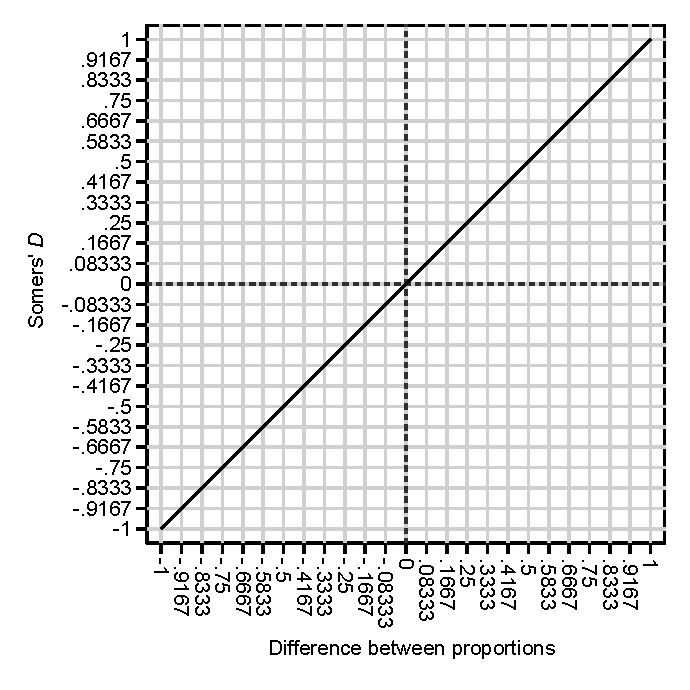
\includegraphics{diffprop.pdf}
\end{figure}

\begin{figure}[htbp]
\caption{Somers'~$D$ and hazard ratio in the two--sample constant hazard ratio model.}
\label{figure:figseq2}
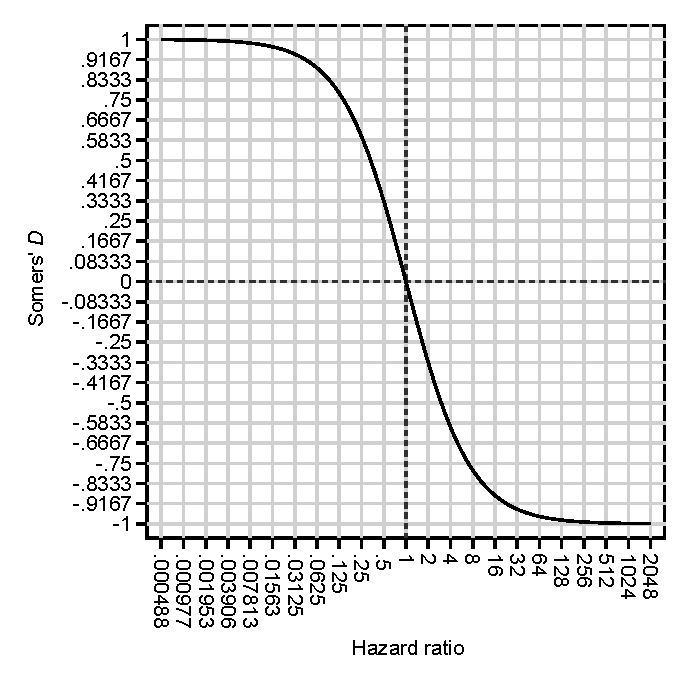
\includegraphics{hazrat.pdf}
\end{figure}

\begin{figure}[htbp]
\caption{Somers'~$D$ and mean difference in SDs in the two--sample equal--variance Normal model.}
\label{figure:figseq3}
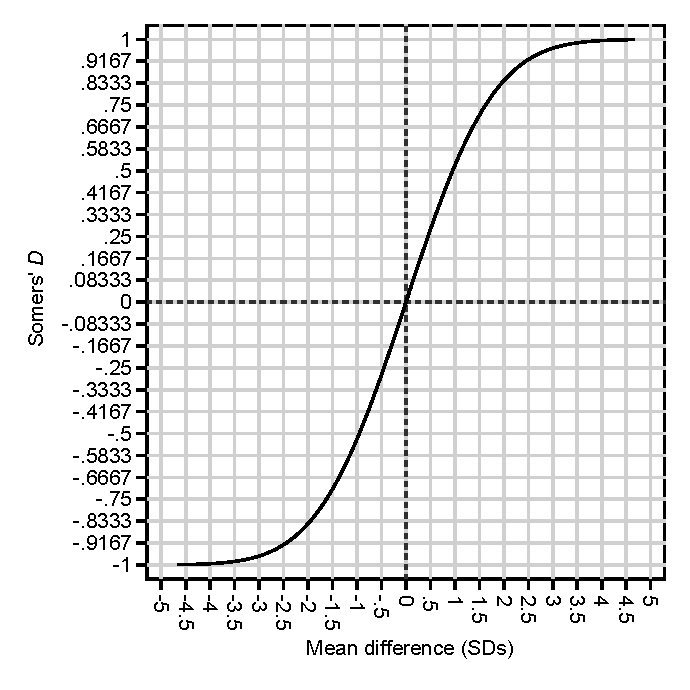
\includegraphics{delta.pdf}
\end{figure}

\begin{figure}[htbp]
\caption{Somers'~$D$ and interquartile odds ratio in the two--sample equal--variance Normal model.}
\label{figure:figseq5}
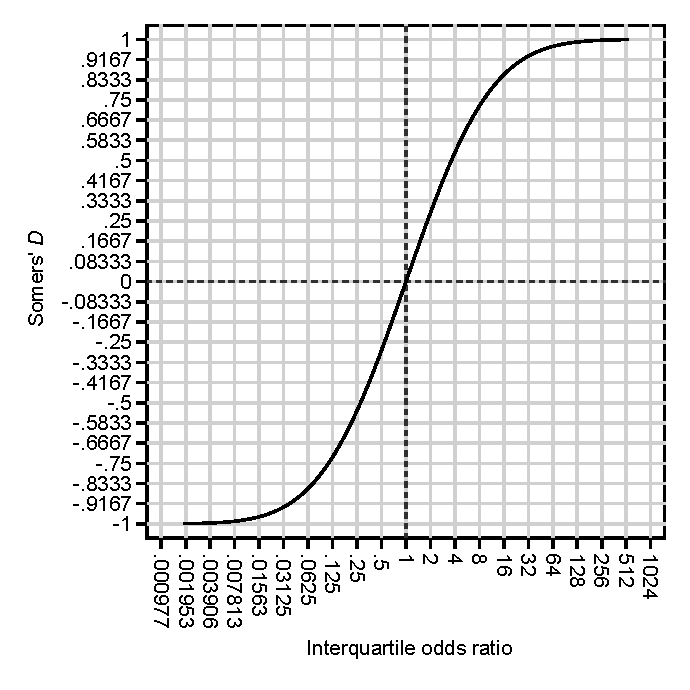
\includegraphics{iqor.pdf}
\end{figure}

\begin{figure}[htbp]
\caption{Interquartile odds ratio and Harrell's~$c$ in the two--sample equal--variance Normal model.}
\label{figure:figseq6}
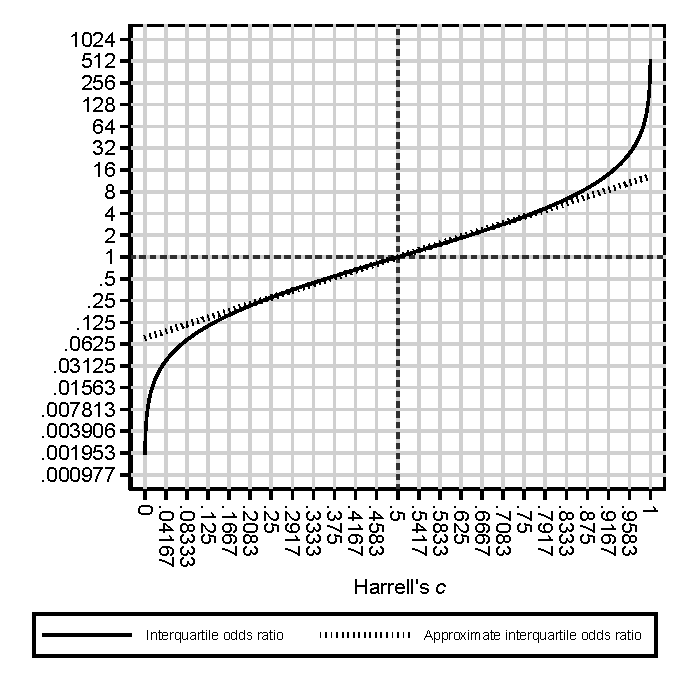
\includegraphics{iqor_c.pdf}
\end{figure}

\begin{figure}[htbp]
\caption{Somers'~$D$ and Pearson correlation in the bivariate Normal model.}
\label{figure:figseq4}
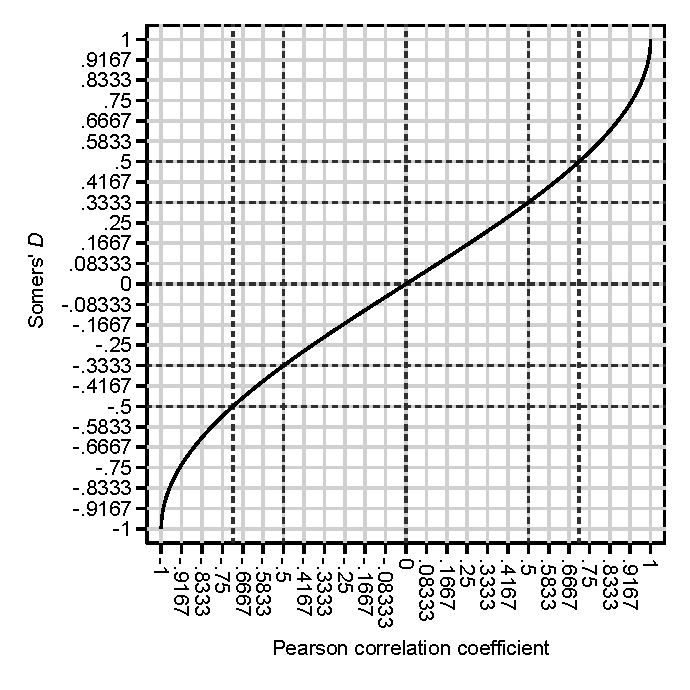
\includegraphics{rho.pdf}
\end{figure}

\end{document}               % End of document.
